\section{Preprocessing}

Describe cleaning, resizing, normalization, tokenization, padding, augmentation, invalid annotation handling, and the input tensor shape(s).

\begin{table}[H]
    \centering
    \caption{Preprocessing pipeline.}
    \label{tab:preprocessing}
    \begin{tabularx}{\textwidth}{@{}lXX@{}}
        \toprule
        Stage & Operation & Configuration \\
        \midrule
        Cleaning & TODO & TODO \\
        Transformation & TODO & TODO \\
        Normalization & TODO & TODO \\
        Augmentation & TODO & TODO \\
        Tensor shape & TODO & TODO \\
        \bottomrule
    \end{tabularx}
\end{table}

\begin{figure}[H]
    \centering
    % Suggested image filename: graphics/preprocessed-batch.png
    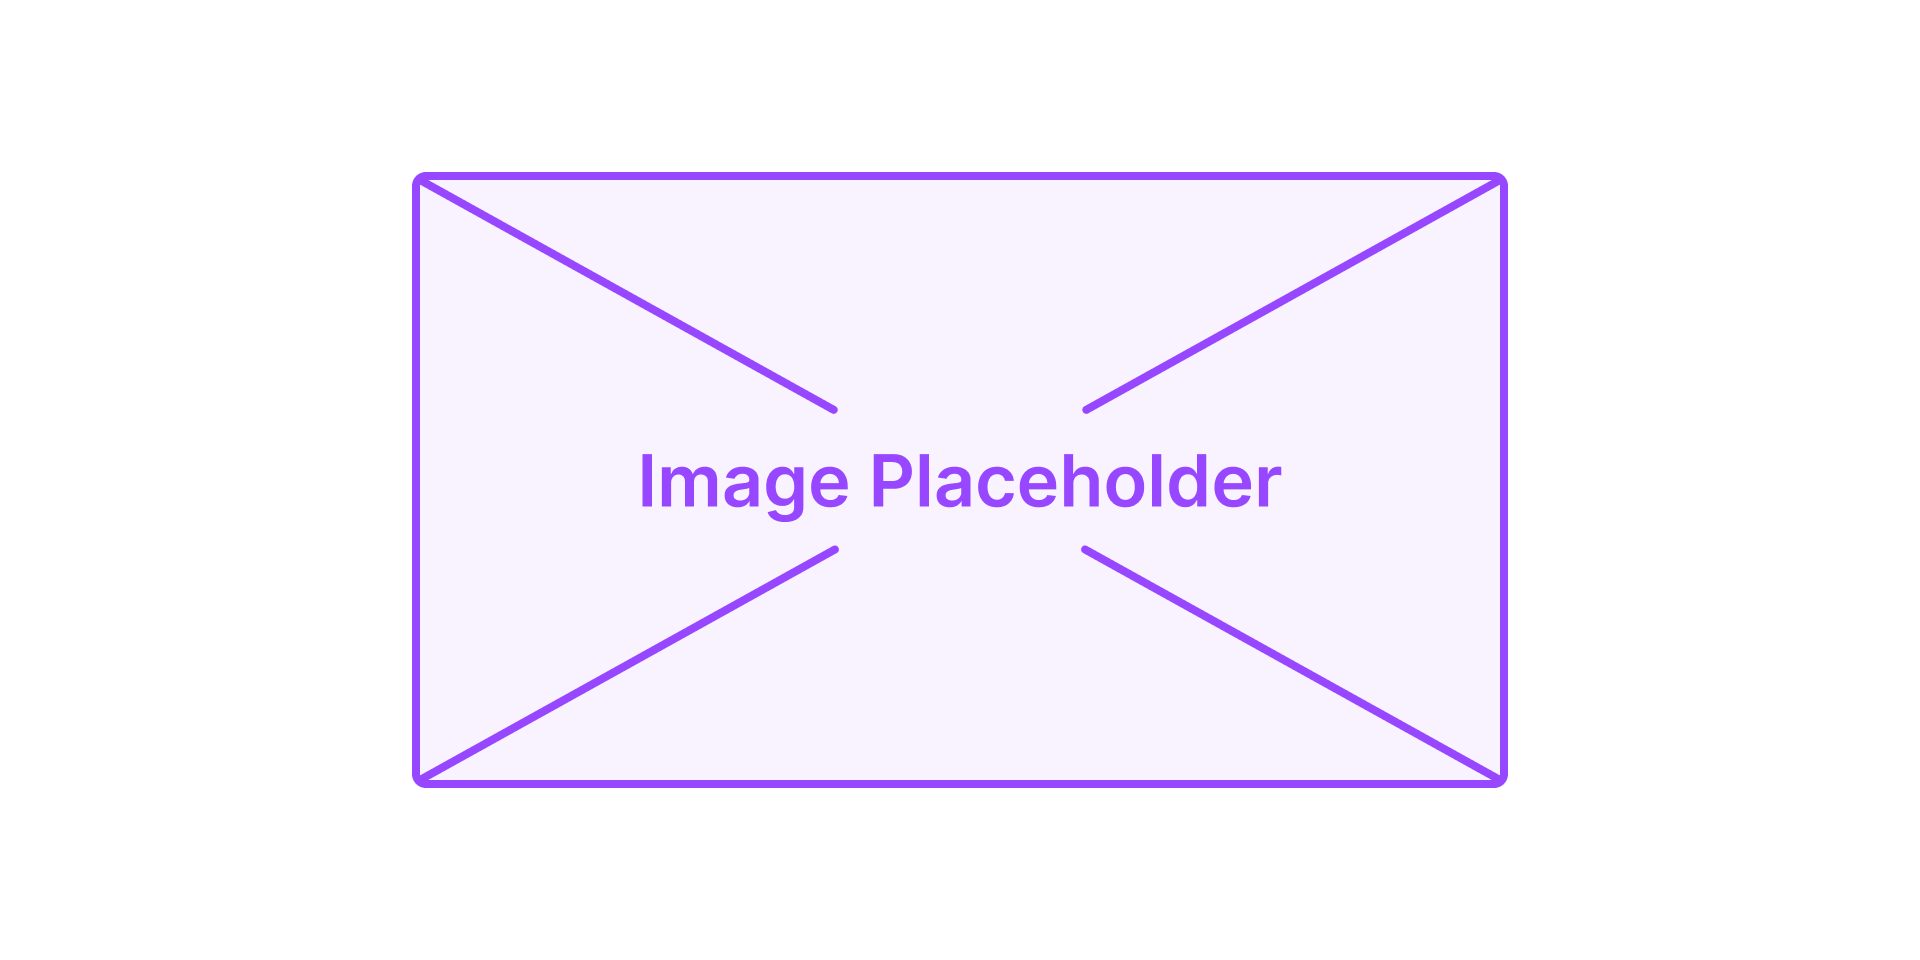
\includegraphics[width=0.9\textwidth]{graphics/placeholder.png}
    \caption{Example batch after preprocessing.}
    \label{fig:preprocessed-batch}
\end{figure}
